\section{The elephant walk near its crossing}\label{sec:shape}

We now look at the whole law of $A_n$ near the crossing
(Figure~\ref{fig:shape}). Unless stated otherwise, $n\ge64$,
$0<\varepsilon\le\frac14$ and $x=n\varepsilon\ge1$. Recall that
$\Prob(A_n=n-m)=\frac12[f_n(m)+f_n(n-m)]$. Some numerical statements also use
odd $n$, and there $x_n$ is the value of $x$ at which the 2 central bins are as
likely as the ends (it is unique by Proposition~\ref{prop:mlr}). For a mode
$a^*\ge n/2$ of the law of $A_n$ we put $m^*=n-a^*$, and $m_h$ is the largest
mode of $f_n$.

\subsection{Families and the first flip}

For $k_0\ge1$ let $(M^{[k_0]}_k)_{k\ge k_0}$ be the Markov chain with
$M^{[k_0]}_{k_0}=0$ and the transition probabilities $r_k(b)$ of $M$. So
$M^{[1]}$ has the law of $M$. We write $Y_d=M^{[1]}_d$, and
$Z^{(j)}_t=M^{[j-1]}_t$ for $j\ge2$ and $t\ge j-1$. In a random recursive tree
on $[n]=\{1,\dots,n\}$, vertex $k+1$ is joined to a uniform vertex of $[k]$,
independently for $k=1,\dots,n-1$. We write $\mathcal T_v$ for the subtree of
$v$, that is, $v$ and its descendants, and we call it the family of $v$. A
single flip at $v$ turns every step of its family.

\begin{lemma}[tree and marks]\label{lem:tree}
Let $\mathcal T$ be the tree on $[n]$ in which the parent of $k+1$ is $U_k$.
For $2\le v\le n$ let $\mu_v=1$ if step $v$ flips the step it copies, and
$\mu_v=0$ otherwise. Then $\mathcal T$ is a random recursive tree, the marks
$\mu_v$ are i.i.d.\ Bernoulli$(\varepsilon)$ and independent of $\mathcal T$,
and $X_v=X_1(-1)^{\sigma(v)}$, where $\sigma(v)$ is the number of marks on the
path from $v$ to the root, the root excluded. So $M_n=\#\{v:\sigma(v)\text{
odd}\}$. If the marks on $2,\dots,k_0$ are set to $0$, then the number of odd
vertices in $[k]$, $k\ge k_0$, is a copy of the chain $M^{[k_0]}$.
\end{lemma}

\begin{proof}
The parent $U_k$ of $k+1$ is uniform on $[k]$ and independent of the earlier
choices, and the marks are the flip indicators. The path from $k+1$ to the root
is $k+1$ followed by the path from $U_k$, so
$\sigma(k+1)=\mu_{k+1}+\sigma(U_k)$ and, by induction on $k$,
$X_{k+1}=X_{U_k}(-1)^{\mu_{k+1}}=X_1(-1)^{\sigma(k+1)}$. Now set
$\mu_2=\dots=\mu_{k_0}=0$. If $b$ of the vertices in $[k]$ are odd, $k\ge k_0$,
then $k+1$ is odd with conditional probability $(1-\varepsilon)\frac
bk+\varepsilon(1-\frac bk)=r_k(b)$, whatever else is known about $[k]$.
\end{proof}

The coupling with a random recursive tree is due to
K\"ursten~\cite{kursten2016}, who uses bond percolation with retention
probability $1-2\varepsilon$. The marks above give the same law of the walk.
For $k\ge v$, if
$\mathcal T_v$ contains $s$ of the vertices in $[k]$, then $k+1$ joins
$\mathcal T_v$ with probability $s/k$. This is the urn of Lemma~\ref{lem:urn},
so $\lvert\mathcal T_v\rvert$ has the law $\beta_v$ and mean $n/v$, and on
average there are $n/(d(d+1))$ families of size $d$. If $v$ is the only marked
vertex, the odd vertices are those of $\mathcal T_v$. Two or more marks have
probability $O(\varepsilon^2)$, and no mark gives $M_n=0$. So at fixed $n$ the
part of $f_n(m)$ of first order in $\varepsilon$ is exactly
$\varepsilon\sum_v\beta_v(m)=x/(m(m+1))$, for $1\le m\le n-1$ (at $m=h$ this
is $c_1\varepsilon$ of Proposition~\ref{prop:first-mutation}). This is also
proved in Lean (Section~\ref{sec:verify}).

\begin{lemma}[splitting]\label{lem:split}
Let $\mathcal T$ be a random recursive tree on $[n]$, let $2\le v\le n$ and let
$S\subseteq[n]$ with $\min S=v$. Given that $\mathcal T_v$ has vertex set $S$,
the restrictions of $\mathcal T$ to $S$ and to $[n]\setminus S$, relabeled in
increasing order, are independent random recursive trees. They are independent
of the parent of $v$, which is uniform on $[v-1]$.
\end{lemma}

\begin{proof}
The tree $\mathcal T$ is uniform over the $(n-1)!$ increasing trees on $[n]$.
Its family $\mathcal T_v$ has vertex set $S$ exactly when every $u\in
S\setminus\{v\}$ has its parent in $S$ and every $u\notin S$ with $u\ge2$ has
its parent outside $S$. So, given this event, each element of $S$ other than
$v$ picks its parent freely among the smaller elements of $S$, $v$ picks any
element of $[v-1]$, and each element of $[n]\setminus S$ other than $1$ picks
freely among the smaller elements of $[n]\setminus S$. This is the claim.
\end{proof}

\begin{lemma}[the first flip]\label{lem:firstmark}
Let $V=\min\{v\ge2:\mu_v=1\}$, with $V=\infty$ if there is no mark, and let
$D=\lvert\mathcal T_V\rvert$. Then
$\Prob(V=j,\,D=d)=\varepsilon(1-\varepsilon)^{j-2}\beta_j(d)$, and for $m\ge1$
\[
 f_n(m)=\sum_{j=2}^n\varepsilon(1-\varepsilon)^{j-2}\sum_{d=1}^{n-j+1}
 \beta_j(d)\,\Prob\bigl(d-Y_d+Z^{(j)}_{n-d}=m\bigr),
\]
where $Y_d$ and $Z^{(j)}_{n-d}$ are independent.
\end{lemma}

\begin{proof}
Marks and tree are independent, which gives the law of $(V,D)$. Condition on
$V=j$ and on the vertex set $S$ of $\mathcal T_j$, with $\lvert S\rvert=d$. The
marks on $j+1,\dots,n$ are still i.i.d., and by Lemma~\ref{lem:split} the trees
on $S$ and on $[n]\setminus S$ are independent random recursive trees. The
vertices $1,\dots,j-1$ carry no mark, so $j$ is odd, and $u\in S$ is odd
exactly when the path from $u$ up to $j$, with $j$ excluded, has an even number
of marks. So by Lemma~\ref{lem:tree} for the tree on $S$ rooted at $j$, the
number of odd vertices in $S$ has the law of $d-Y_d$. Paths from outside $S$
stay outside $S$, and the tree on $[n]\setminus S$ has the unmarked vertices
$1,\dots,j-1$ first. So by Lemma~\ref{lem:tree} its odd count has the law of
$Z^{(j)}_{n-d}$. The 2 counts are independent, and their law depends on $S$
only through $d$. Sum over $j$ and $d$, and note that $M_n=0$ if there is no
mark.
\end{proof}

So the first flip turns its whole family except the steps of that family
that flip back, and the rest of the tree is a walk whose first $j-1$ steps
agree with $X_1$. Only the law of each pair $(Y_d,Z^{(j)}_{n-d})$ enters the
lemma. So from now on $(Y_d)_{d\ge1}$ is one path of $M^{[1]}$ and
$(Z^{(j)}_t)_{t\ge j-1}$ one path of $M^{[j-1]}$, independent of each other
and of $(V,D)$.

\begin{lemma}[unimodality given the first step]\label{lem:unimodal}
The function $f_n$ is unimodal.
\end{lemma}

This is shown in the proof of Theorem~1.1 of Gu\'erin, Laulin, Raschel and
Simon~\cite{glrs2025}, for every $n$ and every memory parameter
$p=1-\varepsilon$, and it is also proved in Lean
(Section~\ref{sec:verify}). So $f_n$ is nondecreasing on $\{0,\dots,m_h\}$
and nonincreasing on $\{m_h,\dots,n\}$.

\subsection{The end and its neighbor}

Bin $n-1$ needs one flip that is never copied, and a flip at step $j$ is never
copied with probability about $j/n$. Summing $\varepsilon j/n$ over $j$ gives
about $x/2$, so the end should fall below its neighbor once $x>2$.

\begin{theorem}[endpoint dip]\label{thm:dip}
Let $n\ge3$ and $0<\varepsilon\le\frac12$, and put $\rho_1=\Prob(A_n=n-1)/E_n$.
Then
\[
 \frac{x}{2(1-\varepsilon)}<\rho_1\le\frac{x(1+1/n)^2}{2-3\varepsilon}+\frac{\varepsilon}{1-\varepsilon}.
\]
Hence the end is strictly below its neighbor if $x\ge2(1-\varepsilon)$, and
strictly above it if the right side is below $1$.
\end{theorem}

\begin{proof}
By Lemma~\ref{lem:erw-reduction}, $\rho_1=\bigl(f_n(1)+f_n(n-1)\bigr)/f_n(0)$
with $f_n(0)=(1-\varepsilon)^{n-1}$. On the event $M_n=1$ the chain first moves
up from time $j-1$ to time $j$, for some $2\le j\le n$, and then stays at $1$.
Since $r_t(0)=\varepsilon$ and $1-r_k(1)=(1-\varepsilon)(1-c/k)$ with
$c=(1-2\varepsilon)/(1-\varepsilon)\in[0,1]$,
\[
 f_n(1)=\varepsilon(1-\varepsilon)^{n-2}\sum_{j=2}^nP_j,\qquad
 P_j=\prod_{k=j}^{n-1}\Bigl(1-\frac ck\Bigr).
\]
Since $c\le1$, $P_j\ge\prod_{k=j}^{n-1}(1-1/k)=(j-1)/(n-1)$, and these lower
bounds sum to $n/2$. So $f_n(1)/f_n(0)\ge x/(2(1-\varepsilon))$. Next,
$1-c/k\le e^{-c/k}$ and $\sum_{k=j}^{n-1}1/k\ge\log(n/j)$ give $P_j\le(j/n)^c$.
As $(t/n)^c$ is nondecreasing in $t$,
\[
 \sum_{j=2}^nP_j\le\int_2^{n+1}\Bigl(\frac tn\Bigr)^c dt
 \le\frac{n(1+1/n)^{c+1}}{c+1}\le\frac{n(1+1/n)^2(1-\varepsilon)}{2-3\varepsilon},
\]
using $c\le1$ and $1/(c+1)=(1-\varepsilon)/(2-3\varepsilon)$. So
$f_n(1)/f_n(0)\le x(1+1/n)^2/(2-3\varepsilon)$. Finally, $M_n=n-1$ needs an up
move at every time. The first has probability $r_1(0)=\varepsilon$, and the one
at time $k\ge2$ has probability
$r_k(k-1)=1-\varepsilon-(1-2\varepsilon)/k\in[\frac12,1-\varepsilon]$. So
$0<f_n(n-1)\le\varepsilon(1-\varepsilon)^{n-2}$. This makes the lower bound
strict and gives the term $\varepsilon/(1-\varepsilon)$.
\end{proof}

\begin{corollary}[the dip at the crossing]\label{cor:dip}
Let $n\ge4$ be even and suppose that $x_n\ge2(1-\varepsilon_n)$. Then at the
crossing $E_n=C_n<\Prob(A_n=n-1)$, and the law of $A_n$ is not unimodal.
\end{corollary}

\begin{proof}
By Proposition~\ref{prop:mlr}, $\varepsilon_n<\frac12$, so
Theorem~\ref{thm:dip} gives $\Prob(A_n=n-1)>E_n=C_n$. Suppose the law is
nondecreasing on $\{0,\dots,a_0\}$ and nonincreasing on $\{a_0,\dots,n\}$. It
is symmetric about $h$, so we may replace $a_0$ by $n-a_0$ and assume
$a_0\le h$. Then
$\Prob(A_n=a)\le C_n$ for every $a\ge h$, including $a=n-1$, which is a
contradiction.
\end{proof}

The hypothesis $x_n\ge2(1-\varepsilon_n)$ holds for every even $n\ge1688$.
To see this, take $\varepsilon=2/n$. Then $\varepsilon(1+\log n)\le\frac1{100}$,
so Theorem~\ref{thm:erw-bounds}(b) gives
$C_n\le\frac8{n(n+2)}n^{4/n}e^{10400/n}$. The right side decreases in $n$ and
is below $1.4\cdot10^{-3}$ at $n=1688$. Since $\log(1-y)\ge-y-y^2$ for
$0\le y\le\frac12$, we also have
$E_n=\frac12(1-\frac2n)^{n-1}\ge\frac12e^{-2-2/n}>0.06$. So $C_n<E_n$ at
$\varepsilon=2/n$, and Proposition~\ref{prop:mlr} gives $\varepsilon_n>2/n$.
Hence $x_n>2\ge2(1-\varepsilon_n)$. A computation shows that the hypothesis
also holds for every $8\le n<1688$. So Corollary~\ref{cor:dip} holds for
every even $n\ge8$, and below $n=1688$ it is computer-assisted. By
Lemma~\ref{lem:unimodal} the law of $A_n$ is a mixture of 2 unimodal laws
with different modes, as is the limit law in~\cite[eq.~(1)]{glrs2025}.

\begin{figure}[t]
\centering
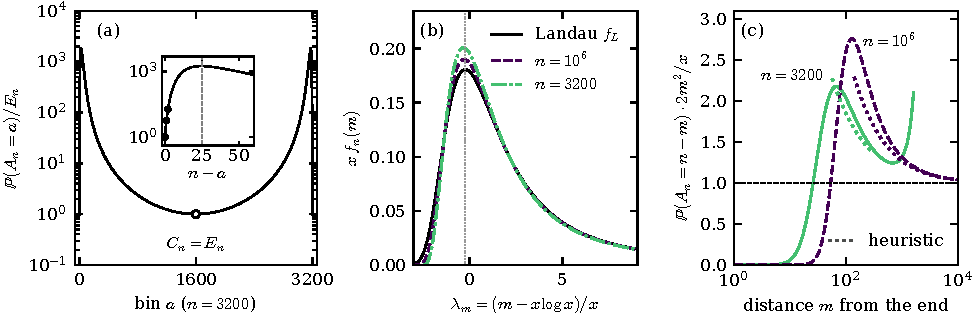
\includegraphics[width=\textwidth]{figures/shape}
\caption{The elephant walk at its crossing. (a) The law of $A_n$ at
$n=3200$ and its crossing $x=11.5468$, divided by the end $E_n$. The center
equals the end, and the law rises from each end to a mode and falls to the
center. The inset shows the last 60 bins, with dots at bins $n$, $n-1$ and
$n-2$. The end is below its neighbor, and the modes are 25 steps from each end
(dashed). (b) The law of $M_n$, scaled as $xf_n(m)$, against
$\lambda_m=(m-x\log x)/x$, with the Landau density $f_L$. The dotted line is
its mode $\lambda_0$. (c) The tail $\Prob(A_n=n-m)$ divided by $x/(2m^2)$. The
dashed line is the limit 1 of Theorem~\ref{thm:profile}, and the dotted
curves are the heuristic correction $1+x(2\log m+2\gamma-3)/m$ for
$2x\log x\le m\le n/x$. The rise of the $n=3200$ curve near $m=n/2$ is the
mirror term $f_n(n-m)$. At $n=10^6$ we use $x=g_n=22.4407$.}
\label{fig:shape}
\end{figure}

\subsection{The bulk}

Let $\CP_n$ be the law of $\sum_{d=1}^{n-1}dN_d$, where the $N_d$ are
independent Poisson variables with means $x/(d(d+1))$. On average
$x/(d(d+1))$ flipped vertices have a family of size $d$. If no 2 flips fall in
the same family, which is likely when $x^2\log n/n$ is small, then $M_n$ is the
total size of the flipped families, and this is close to a compound Poisson
sum.

\begin{remark}[compound Poisson and Landau limits, proofs omitted]\label{rem:bulk}
For $n\ge2$ and $0<\varepsilon\le\frac14$, Fourier inversion, the tree of
Lemma~\ref{lem:tree} and the Efron--Stein inequality~\cite{efronstein1981}
give
$\sup_m\lvert f_n(m)-\CP_n(m)\rvert\le\delta_B:=\frac{x^2\log n}{n}
+\frac{4x^2}{n}e^{4x^2/n}+\frac{4x^2(H_n^2+H_n)}{n}$. Let $f_L$ be the Landau
density, with $\int e^{-u\lambda}f_L(\lambda)\,d\lambda=u^u$ for $u>0$, and put
$\lambda_m=(m-x\log x)/x$. Families of size $d$ are flipped at rate about
$x/d^2$, so the families of size up to about $x$ add up to nearly $x\log x$,
and the few families of size of order $x$ give fluctuations of order $x$.
Under the standing assumptions of this section, comparing characteristic
functions then gives $\sup_m\lvert xf_n(m)-f_L(\lambda_m)\rvert\le
C(\frac{1+\log x}x+\frac xn)+x\delta_B$ with an absolute constant $C$. So
$(M_n-x\log x)/x$ tends to the Landau law when $x\to\infty$ and
$x^3\log^2n/n\to0$, in particular at the crossing. We omit the details of
these 2 bounds. At $n=10^6$ and $x=22.4407$ the bound $\delta_B$ is still about
$0.46$, but there $\lvert f_n(m)/\CP_n(m)-1\rvert\le3.5\cdot10^{-4}$ for
$1\le m\le10^4$. At every tested crossing $m^*$ equals the mode of $\CP_n$. If
$f_L''(\lambda_0)<0$ at the mode $\lambda_0=-0.2228$ of $f_L$, then the
unimodality of $f_L$~\cite{yamazato1978} and the bound above give
$m^*=x\log x+\lambda_0x+O(\sqrt{x\log x})$ at the crossing for large $n$. We
computed $f_L''(\lambda_0)=-0.0789$ by quadrature but did not certify its
sign.
\end{remark}

\subsection{The tail}

\begin{theorem}[the tail]\label{thm:profile}
Let $n$ be even, and let $x=n\varepsilon\ge1$ depend on $n$ with
$x\log^2n/n\to0$. Let $\omega_n\to\infty$ with $\omega_nx\log^2(x+1)=o(n)$, and
let $\delta'_n\to0$. Then
\[
 f_n(m)=\frac{x}{m(m+1)}\bigl(1+o(1)\bigr)\qquad\text{and}\qquad
 \Prob(A_n=n-m)=\frac{x}{2m^2}\bigl(1+o(1)\bigr),
\]
uniformly for $\omega_nx\log^2(x+1)\le m\le\delta'_nn$.
\end{theorem}

In the proof (Appendix~\ref{app:shape}) the lower bound uses the first flipped
family, which has size $m$ with probability about $x/(m(m+1))$ by
Lemma~\ref{lem:B-D}, while the other flips change the count only by a relative
amount of order $x\log m/m$. For the upper bound we show $\Prob(M_n\ge
m)\le\frac xm(1+O(x\log^2m/m))$, and the unimodality of $f_n$ turns this into a
local bound. The mirror term $f_n(n-m)$ is at most $C_n=O(x/n^2)$ by
Lemma~\ref{lem:unimodal} and Theorem~\ref{thm:erw-bounds}(b), so bin $n-m$ is
reached through a family of size $m$ only when $X_1=+1$, and this gives the
constant $\frac12$. At $n=10^6$, $x=22.4407$ and $m=10^4$ the exact ratio
$\Prob(A_n=n-m)/(x/m^2)$ is $0.51889$. At moderate $m$, $\CP_n$ suggests $f_n(m)\,m(m+1)/x\approx1+x(2\log m+2\gamma-3)/m$, and
this factor is still about $2$ near $m=70$ when $n=1600$.

\subsection{The center}

\begin{theorem}[shape at the crossing]\label{thm:shape}
There are absolute constants $C_{\rm w}$ and $n_0$ with the following
property. Let $n\ge n_0$ be even with $x_n\in[2,n^{1/4}]$. Then at the
crossing $\Prob(A_n=a)>C_n$ for every $1\le a\le n-1$ with
$\lvert a-h\rvert\ge C_{\rm w}(nx_n\log n)^{1/2}$.
\end{theorem}

By Theorem~\ref{thm:erw-crossing}, $x_n\in[2,n^{1/4}]$ for large $n$, so at the
crossing the window has width of order $n^{1/2}\log n$.

\begin{proof}
Write $x=x_n$ and $\varepsilon=\varepsilon_n$, so that $C_n=E_n$. By
symmetry we take $a=n-m$ with $1\le m\le h$, and put $t=h-m$. Since $2\le
x\le n^{1/4}$, every error term below is bounded by a function of $n$ alone,
and we take $n$ large. Put
$\Pi(m)=\frac12\bigl[\frac1{m(m+1)}+\frac1{(n-m)(n-m+1)}\bigr]$, so that
$x\Pi(h)=\frac{4\varepsilon}{n+2}$. As $\varepsilon(1+\log n)\to0$,
Theorem~\ref{thm:erw-bounds}(b) gives $C_n\le x\Pi(h)(1+\eta)$ with
$\eta=n^{2\varepsilon}e^{5200\varepsilon}-1$. Put $u=\varepsilon(2\log n+5200)$.
Then $u\le\frac12$ for large $n$, and $e^u-1\le2u$ for $0\le u\le\frac12$, so
$\eta\le2u\le10^4\varepsilon\log n$.

If $m\le m_h$, then $f_n(m)\ge f_n(1)$ by Lemma~\ref{lem:unimodal}. The proof
of Theorem~\ref{thm:dip} gives $f_n(1)\ge\frac x{2(1-\varepsilon)}f_n(0)$, and
$f_n(0)=2E_n=2C_n$. So $\Prob(A_n=n-m)\ge\frac12f_n(m)\ge\frac
x{2(1-\varepsilon)}C_n>C_n$.

If $m_h<m\le n/8$, then $f_n(m)\ge f_n(k)$ with $k=\lfloor n/8\rfloor$, by
Lemma~\ref{lem:unimodal}. Proposition~\ref{thm:B-local-lower}(a) at $k$ gives
$f_n(k)\ge\frac{x}{k(k+1)}(1-O(\frac{x\log n}n))$. So
$\Prob(A_n=n-m)\ge\frac{32x}{n(n+8)}(1-o(1))$, which exceeds
$\frac{4x}{n(n+2)}(1+\eta)\ge C_n$.

If $n/8<m\le h$, then $m$ and $n-m$ are at least $n/8$, and
Proposition~\ref{thm:B-local-lower} at $m$ and at $n-m$ gives
$\Prob(A_n=n-m)\ge x\Pi(m)(1-\bar e)$ with $\bar e=O(x\log n/n)$. Put $N=n+1$
and $s=2t/N$, so that $m+\frac12=\frac N2(1-s)$ and $n-m+\frac12=\frac
N2(1+s)$. Since $\frac1{k(k+1)}\ge(k+\frac12)^{-2}$ and
$\Pi(h)=\frac1{h(h+1)}=(\frac N2)^{-2}(1-N^{-2})^{-1}$, we get
$\frac{\Pi(m)}{\Pi(h)}\ge\frac12[(1-s)^{-2}+(1+s)^{-2}](1-N^{-2})\ge(1+3s^2)(1-N^{-2})$,
because $\frac12[(1-s)^{-2}+(1+s)^{-2}]=\sum_{k\ge0}(2k+1)s^{2k}$. With $b=\bar
e+N^{-2}\le\frac12$ this gives $\Prob(A_n=n-m)\ge x\Pi(h)(1+3s^2)(1-b)\ge
x\Pi(h)(1+\frac32s^2-b)$, which exceeds $x\Pi(h)(1+\eta)\ge C_n$ as soon as
$\frac32s^2>\eta+b$. Now $\eta+b\le A_2x\log n/n$ for an absolute constant
$A_2$, since $x\ge2$, and $s\ge t/n$. So the condition holds when $t\ge C_{\rm
w}(nx\log n)^{1/2}$ with $C_{\rm w}^2>2A_2/3$.
\end{proof}

The window has this size because, at distance $t$ from $h$, the main term
$x\Pi(m)$ exceeds its value at $h$ by a factor of about $1+12t^2/n^2$, while we
know $C_n$ and the law only up to relative errors of order $x\log n/n$. We did
not compute $C_{\rm w}$ or $n_0$. Inside the window the proof gives nothing,
and closing it needs second differences of the law.

\begin{conjecture}[convexity between the humps]\label{conj:convex}
For every $n\ge10$ and $x=x_n$, the second difference
$\Prob(A_n=a-1)-2\Prob(A_n=a)+\Prob(A_n=a+1)$ is positive for
$2m^*+1\le a\le n-2m^*-1$.
\end{conjecture}

With the symmetry of the law, the conjecture makes the law strictly convex on
$[2m^*,n-2m^*]$, so $h$ is its unique minimizer there (the 2 central bins for
odd $n$). The next corollary shows that $m^*=o(n)$ at the crossing.

\begin{corollary}[the modes]\label{cor:modes}
For large even $n$ the modes $a^*$ of the law of $A_n$ at the crossing
satisfy $\min(a^*,n-a^*)=O(x_n\log^2x_n)$.
\end{corollary}

\begin{proof}
Write $x=x_n$ and $\varepsilon=\varepsilon_n$. By
Theorem~\ref{thm:erw-crossing}, $x\sim2\log n$, so for large $n$ the
hypotheses of Theorem~\ref{thm:erw-bounds}(b) and Lemma~\ref{lem:B-mode}
hold. The law is symmetric about $h$, so $m^*=\min(a^*,n-a^*)$ maximizes
$f_n(m)+f_n(n-m)$ over $0\le m\le h$. Lemma~\ref{lem:B-mode} gives $m_h\le h$
for large $n$. So Lemma~\ref{lem:unimodal} and
Theorem~\ref{thm:erw-bounds}(b) give $f_n(n-m)\le f_n(h)=C_n=O(x/n^2)$ for
$m\le h$, and hence $f_n(m^*)\ge f_n(m_h)-C_n$. Let $\ell$ be as in the proof
of Lemma~\ref{lem:B-mode}. Then $f_n(m_h)\ge f_n(\ell)\ge\frac
x{2\ell(\ell+1)}$, so $f_n(m^*)\ge\frac x{4\ell(\ell+1)}$ for large $n$. If
$m^*>m'=\max(m_h,\ell)$, then Lemmas~\ref{lem:B-sandwich}
and~\ref{lem:B-tail} give $(m^*-m'+1)f_n(m^*)\le\Prob(M_n\ge\ell)\le
xH_\ell/\ell$. Hence $m^*\le\max(m_h,\ell)+4(\ell+1)H_\ell$ in every case.
Finally Lemma~\ref{lem:B-mode} gives $m_h=O(x\log^2x)$, and $\ell=O(x\log x)$
and $H_\ell=O(\log x)$.
\end{proof}

So for large even $n$ Theorem~\ref{thm:shape} covers the bins outside
$[2m^*,n-2m^*]$, and the conjecture would make the center the unique interior
minimum. The conjecture holds for every $10\le n\le600$ and for
$n=800,1600,\dots,25600$. On the closed range
$[2m^*,n-2m^*]$ it fails only at the 2 endpoints and only for some $n\le51$.
Heuristically, a concave stretch of $f_n$ far from its mode is added to the
tail $x/(2r^2)$ of the other branch, with $r=n-a$, and the second difference
$3x/r^4$ of this tail beats the concave curvature, which is of order
$x^2/(n^2r^3)$. We leave open the
window around the center, the tail between $x\log x$ and $x\log^2x$, and
effective constants in Theorems~\ref{thm:profile} and~\ref{thm:shape}.
